\documentclass[10pt,oneside,a4paper]{article}
\usepackage[IL2]{fontenc}
\usepackage[utf8]{inputenc}
\usepackage{graphicx}
\usepackage{url} 
\usepackage{hyperref} 

\usepackage{cite}
\usepackage{multirow}

\pagestyle{headings}
\title{Procedural Game Content Generation Using the Wave Function Collapse Algorithm\thanks{Semester project in the subject Methods of engineering work, year 2022/23, management: Ing. Igor Stupavský }}
\author{Martin Dinja\\[2pt]
	{\small Slovak University of Technology in Bratislava}\\
	{\small Faculty of Informatics and Information Technologies}\\
	{\small \texttt{xdinja@stuba.sk}}
}

\date{\small 14.\ december 2022}

\begin{document}

\maketitle

% \tableofcontents

\begin{abstract}
    \begin{center}
        This thesis examines the problem of generating game content using the Wave Function Collapse (WFC) algorithm.
        The algorithm is thoroughly described and its effectiveness in generating game content is demonstrated.
        Additionally, the thesis includes a comparison of the WFC algorithm with other methods of generating game content.
        Through this analysis, the potential of the WFC algorithm as a tool for game content generation is explored.
    \end{center}
\end{abstract}

\section{Introduction}\label{sec:introduction}

% An Introduction to the application of the wave function collapse algorithm for procedural generation of game content.
Procedural content generation (PCG) is a general term for a system that follows some patterns and generates an output based on those patterns.
Its main use case is generating assets or content that would be too time-consuming to create manually.
PCG is mainly connotatively tied to game content generation, but its use cases can be more creative.
Most PCG systems use game-specific assets with game-specific rules and algorithms to generate their content.
A more general application fit for a wide range of games is the Wave Function Collapse algorithm developed by Maxim Gumin~\cite{WFC}.
The Wave Function Collapse (WFC) algorithm is a greedy PCG method that is based on the concept of collapsing a wave function, a mathematical representation of a quantum state.
This method can generate a controlled, consistent and high-quality output from a small set of input patterns.
It has a variety of potential applications, but is most commonly used for generating 2D tile-maps for games.
However, it can also be used to generate 3D models, music, poetry, and more.
WFC's output can only be as good as its input, so it's essential to have a good set of input patterns and rules. 
\newpage
\section{Theory}\label{sec:theory}
% Theoretical background of the wave function collapse algorithm.
As mentioned in the introduction [\ref*{sec:introduction}], the Wave Function Collapse algorithm is based on the concept of collapsing a wave function.
In the context of quantum mechanics, a wave function is a mathematical representation of the quantum state of a system.
It is a function that assigns a complex number to each point in space, representing the amplitude of the wave at that point.
When a wave function is measured, it collapses, meaning that the complex number associated with each point in space is replaced with a single real number, representing the value of the wave function at that point in time.

This concept of wave function collapse is exactly how the WFC algorithm works.
First, we define a set of input patterns and their associated rules.
Next, the algorithm assigns each tile a superposition of all possible patterns.
Then, the algorithm selects the tile with the least superpositions, also known as the least entropy, assigns it a random pattern from its superposition, and collapses its wave function.
This process is repeated, with the algorithm reevaluating the affected tiles and removing any patterns that do not fit the rules at each step.
The algorithm continues until there is no remaining entropy in the tile-map.
Boris explains WFC in more detail in his Wave Function Collapse Explained blog.~\cite{WFCE}.

\section{Extensions}\label{sec:extensions}
Other than the most basic implementation of the algorithm, we also have extensions to the algorithm that allow us to generate more complex content.
For example, we can have a differently shaped grid, different constraints, and ways of looking at those constraints.

\subsection{The Overlap Model}
The most notable extension is the Overlap Model, which is mainly used to generate 2D textures.
Instead of concerning ourselves with adjacency rules for tiles, here we input an image that will act as bout our input pattern and our constraints.
In the overlap model of WFC, the input is divided into overlapping segments (usually a 3$\times$3 pixel group), and the algorithm calculates the likelihood of each possible configuration of the segments.
This allows the algorithm to consider multiple possible configurations for a given input, which can improve the coherence and randomness of the generated patterns.
The overlap model produces a variation of the input pattern.
It is very intuitive to use. However it is also harder to implement, slower, and less flexible than the tiling model.
This extension is not used in this implementation, but it is still worth mentioning.

\subsection{Semi-Automatic Rule System}\label{sec:semi-automatic_rule_system}
Rather of defining every relation to every possible rotation of every tile.
We can use an array of four numbers representing a connection type for each side of the tile. \texttt{[top, right, bottom, left]}.
Only the same connection types are allowed to connect to each other.
The system then automatically generates all the possible rotations of the tile and their connections.
We can also define which tile can connect to which other tile. Making sure that, even if the connection types match, we can still prevent the tiles from connecting to each other if needed.
\begin{figure}[ht]
    \centering
    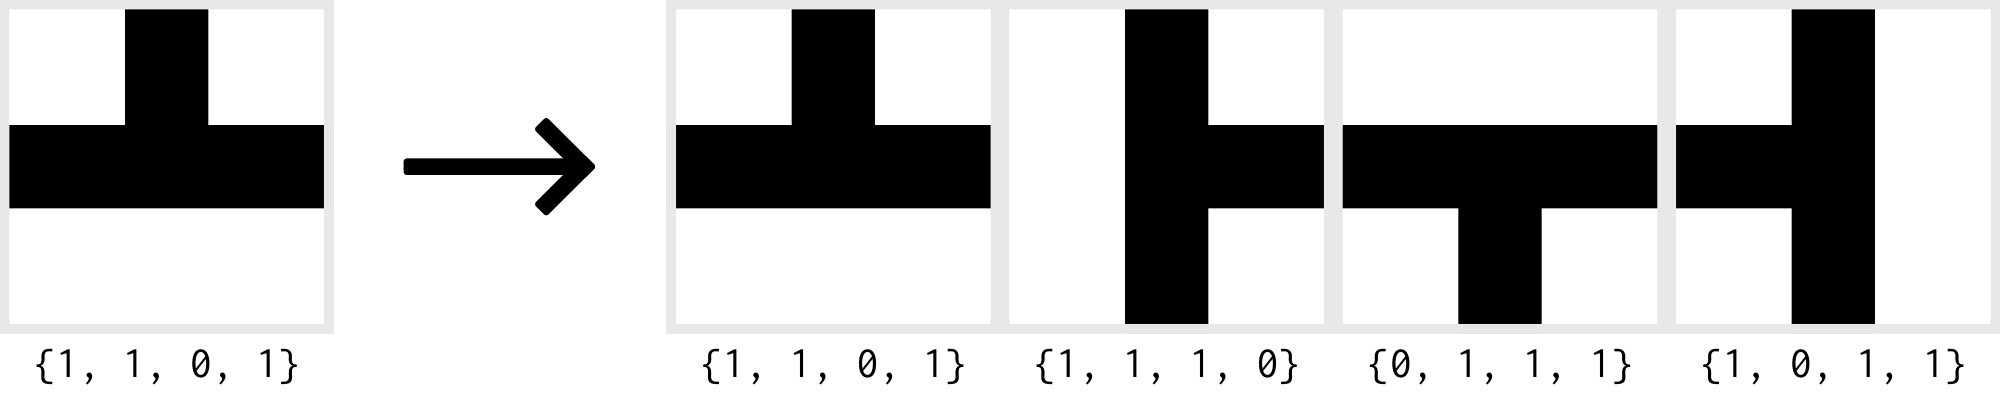
\includegraphics[width=0.8\textwidth]{figures/tile_rotation_example.png}
    \caption{Tile Rotation}\label{fig:tile_rotation_example}
\end{figure}

\section{Algorithm Implementation}\label{sec:implementation}
In this implementation of the WFC algorithm, we use the basic tiling model. Primarily because it can be manually configured with more complex constraints, making it more suitable for game content generation.
We also use the semi-automatic rule system extension mentioned in the previous section [\ref*{sec:semi-automatic_rule_system}].

The central part of the project is the algorithm itself.
It uses the helper, interface, and infrastructure functions to work with the tile grid.
It starts by inferring all the rules with the semi-automatic rule system[\ref*{sec:semi-automatic_rule_system}].
Then it initializes the tile grid and fills each tile's state array with all possible states.
Then the main loop of the algorithm starts.
In the loop, we get the tile with the least entropy, collapse it, and reevaluate all the affected cells.
We evaluate the cells by updating each collapsed cell's neighbors and reevaluating their neighbors until no further changes occur.
Finally, we check if all of the cells have collapsed. If they have, the algorithm halts.
Otherwise, we repeat the loop.
\newline
\begin{figure}[ht]
    \centering
    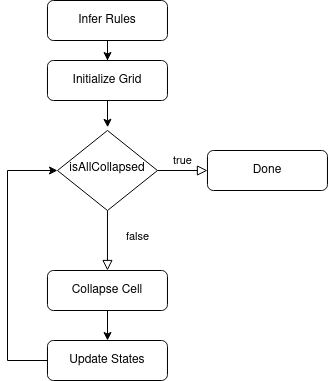
\includegraphics[width=0.5\textwidth]{figures/model_loop_diagram.png}
    \caption{Model Loop Diagram}\label{fig:model_loop_diagram}
\end{figure}

\section{Results}\label{sec:results}
% subsections: examples, performance, conclusions.
With the algorithm implemented, we can now generate tile-maps.
Starting off with a simple example (Figure~\ref{fig:example1}).
\begin{figure}[ht]
    \centering
    
\includegraphics[width=0.5\textwidth]{figures/road_tiles.png}
    \caption{Road Tiles}\label{fig:example1}
\end{figure}

Defining the rules for these tiles, we can generate a 10 by 10 tile-map with the following result (Figure~\ref{fig:example1map}):

\begin{figure}[ht]
    \centering
    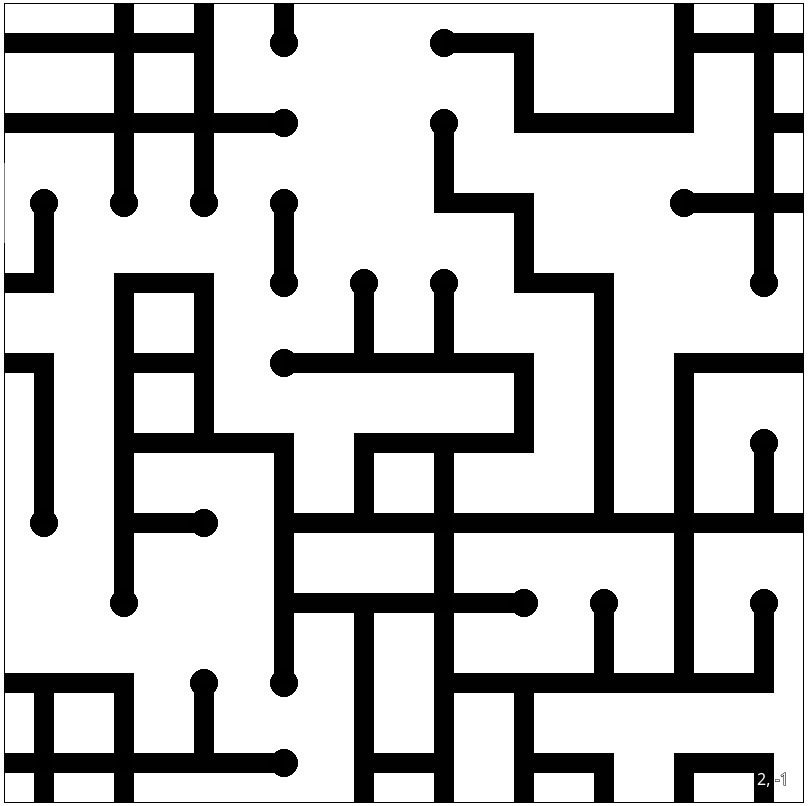
\includegraphics[width=0.35\textwidth]{figures/roads_output.png}
    \caption{Road Output}\label{fig:example1map}
\end{figure}

It works great with simple rules and small tile-maps. 
However, the simplicity of the algorithm makes it prone to failure when confronted with complex rule sets or large grid sizes.
This limitation is a result of the algorithm's inadequate design, which fails to adequately address the challenges posed by these conditions.
Consequently, the algorithm's performance may be compromised, leading to incorrect or unreliable results.
To address these issues, we can optimize the algorithm and augment the rule system to support a broader range of rules.
Possible improvements to the algorithm are discussed in the next section [\ref*{sec:modifications}].
\newline
% Table of the succes rate depending on the size of the grid and the complexity of the rules.
\begin{table}[ht]
    \centering
    \begin{tabular}{|c|cc|}
        \hline
        \multirow{2}{*}{Grid}   & \multicolumn{2}{c|}{Rules} \\ \cline{2-3} 
                                & \multicolumn{1}{c|}{Simple} 
                                & \multicolumn{1}{c|}{Complex} \\ \hline
        \multicolumn{1}{|l|}{10$\times$10} & \multicolumn{1}{l|}{100\%}  & 90\% \\ \hline
        \multicolumn{1}{|l|}{25$\times$25} & \multicolumn{1}{l|}{100\%}  & 78\% \\ \hline
        \multicolumn{1}{|l|}{50$\times$50} & \multicolumn{1}{l|}{100\%}  & 28\% \\ \hline
        \multicolumn{1}{|l|}{75$\times$75} & \multicolumn{1}{l|}{100\%}  & 17\% \\ \hline
        \multicolumn{1}{|l|}{100$\times$100} & \multicolumn{1}{l|}{100\%}  & 5\% \\ \hline
        
    \end{tabular}
    \caption{Success Rate}\label{tab:success_rate}
\end{table}     

As we can see in Table~\ref{tab:success_rate}, the algorithm's performance is highly dependent on the size of the grid and the complexity of the rules.

\newpage
\section{Modifications}\label{sec:modifications}
% Modifications to the algorithm.
The algorithm is characterized by its simplicity and transparency, but it can be adapted to accommodate diverse requirements.
For instance, to achieve a more controlled distribution of tile types, we can assign a weight value to each type.
This weight value can be used to determine the probability that a tile will be collapsed into a specific pattern.
By modifying the algorithm in this way, we can effectively control the distribution of tile types and improve the performance of the algorithm.

WFC can also be enhanced with genetic search, enabling it to generate levels with specific play experiences.
For example, Bailly and Levieux's paper describes a genetic search-based approach to level generation using WFC~\cite{BL22}.

There is also a way to augment the algorithm with the Growing Grid neural network for procedural map generation~\cite{NMBP20}.

We can further control the algorithm by introducing additional constraints, resulting in outputs that appear more human-designed.
For example, Cheng, Han, and Fei's paper describes a constraint-based approach to level generation using WFC~\cite{CHF20}.

The wave function collapse algorithm can be modified in a number of other ways to suit different applications.
The flexibility of the algorithm allows for a range of potential uses and modifications, making it a useful tool in a variety of contexts.

\section{Comparison with other methods}\label{sec:comparison}
% subsections: other methods, pros and cons.

Procedural content generation (PCG) algorithms, like the Wave Function Collapse (WFC) algorithm, have varying strengths and limitations.
Some are better suited for specific tasks, while others are more general.
Comparing these algorithms can be difficult due to their diverse approaches and goals, but a comparison to related methods can still be made.
Examples of such algorithms include model synthesis, Perlin noise, Markov chain algorithms, genetic algorithms, and L-systems.

There are many similarities between WFC and these PCG algorithms, but the main difference is the type of mathematical models used to generate the output.
Although each algorithm can be configured to generate different types of content, they all operate in very different ways.

As we already know, WFC uses a random process known as the ``collapse'' of a wave function to determine which input patterns are selected and combined to create the output.
Its most commonly used for generating 2D tile-maps for games, but can also be applied to other types of content.

Model Synthesis is a constraint-based algorithm mainly used for generating 3D models.
Paul Merrell, the creator of model synthesis has compared the two algorithms in his paper\cite{Mer21}.
\begin{quote}
    \textit{Model synthesis and WFC use nearly the same algorithm and produce similar results. WFC picks cells in a different
order and does not modify in blocks. This causes the algorithm to fail more on some large models.}
\end{quote}

Perlin noise uses a random noise function to generate smooth, natural-looking patterns or textures\cite{PerNoise}.

Markov chain algorithms use statistical models to generate sequences of symbols or events based on the probabilities of their occurrences in the input data.
They can be used to generate a wide range of outputs, including text, music, and images\cite{MCHAIN}.

Genetic algorithms are commonly used to solve optimization problems, and can be applied to a wide range of domains, including game content generation\cite{GeneticAA}.

And L-systems are commonly used to model the growth of plants and other natural systems, and can be applied to generate 2D and 3D graphics, as well as other types of content\cite{LSys}.

Each of these algorithms have their own unique characteristics and capabilities, and can be used in a variety of applications.

\section{Conclusion}\label{sec:conclusion}
In this thesis, we had a brief introduction to PCG algorithms.
We explained in detail how the algorithm works, a way to implemented it, and how it can be modified.
We also showed some examples of the algorithm in action, and compared it to some other PCG algorithms.
In conclusion, WFC is a very theoretically simple algorithm, but it's very powerful and can be used to generate a wide variety of content.
It also has a very simple implementation, and can be easily modified to fit different needs.
The main limitations of basic WFC is that it is computationally intensive and unfit for real-time applications. 
However, it's a great algorithm to start with when learning about PCG\@.
\newpage
\bibliography{lit}
\bibliographystyle{alpha}

\end{document}
